\section{Results and Discussion}
The results from running the failure scenarios on the three platforms are summarized in table \ref{fig:failurescenariosresult}.
\begin{table}[h]
	\centering
	\begin{tabular}{|l|l|l|l|}
		\hline
		& Apache Kafka & Apache Pulsar & NATS Streaming \\ \hline
		\textit{event-generator-crash}  & Exactly-once & Exactly-once  & At-least-once  \\ \hline
		\textit{stream-processor-crash} & Exactly-once & Exactly-once  & At-least-once  \\ \hline
		\textit{view-generator-crash}   & Exactly-once & Exactly-once  & Exactly-once   \\ \hline
		\textit{duplicated-consumer}    & Exactly-once & Exactly-once  & Not applicable \\ \hline
	\end{tabular}
	\caption{Summary of 4 failure scenarios.}
	\label{fig:failurescenariosresult}
\end{table}

As expected, the transactional features of Kafka and Pulsar help ensure exactly-once semantics in the case of \emph{event-generator-crash} and \emph{stream-processor-crash} failure scenarios. On the other hand, NATS Streaming can only provide at-least-once guarantee in these scenarios.  

With the \emph{view-generator-crash} scenario, exactly-once semantics is guaranteed with all three platforms. Nevertheless, this is only resulted from the support of transaction on the sink relational database and requires manual implementation on the application level to bridge the gap between the two data systems. 

Regarding the \emph{duplicated-consumer} failure scenario, the locking mechanisms of the transactions on Kafka and Pulsar are effective to guarantee exactly-once semantics even when a message is delivered and processed by two different stream processor instances when partition reassignment occurs. 

\begin{figure}[h]
	\centering
	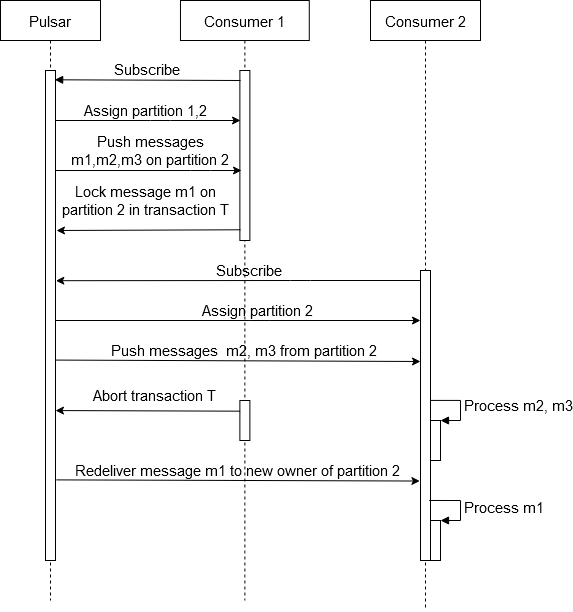
\includegraphics[width=11cm]{images/pulsar-transaction-out-of-order.png}
	\caption{Pulsar transaction can result in out-of-order processing of messages when transaction is aborted.}
	\label{fig:pulsaroutofordertransaction}
\end{figure}

However, the transaction feature on Pulsar can potentially lead to out-of-order processing of messages on the same partition. With the Pulsar transaction, when a message in locked by a consumer instance by being acknowledged in a transaction, this message cannot be redelivered to another consumer instance or cannot be acknowledged by other consumers if it is already delivered to their local queues. However, subsequent messages on the same partition can still be processed and acknowledged by other consumers. In the scenario depicted in figure \ref{fig:pulsaroutofordertransaction}, when partition is reassigned to consumer 2 when it joins the subscription, message m1 is already locked by consumer 1 and therefore will not be pushed to consumer 2. However, when consumer 1 fails to complete the transaction, message m1 will return to unacknowledged state and will be redelivered and processed again. This causes message m1 to be processed out-of-order after message m2 and m3 even though they are on the same partition where order is guaranteed.

Moreover, this mechanism of Pulsar to let consumers race to lock messages when they have the same messages buffered locally can lead to unexpected behaviors during runtime when a partition is not guaranteed to be consumed by only one application instance at any time. Nevertheless, since this transaction feature of Pulsar is still actively developed and refined in the technical review phase, this problem could be soon resolved in future releases. 

\begin{figure}[h]
	\centering
	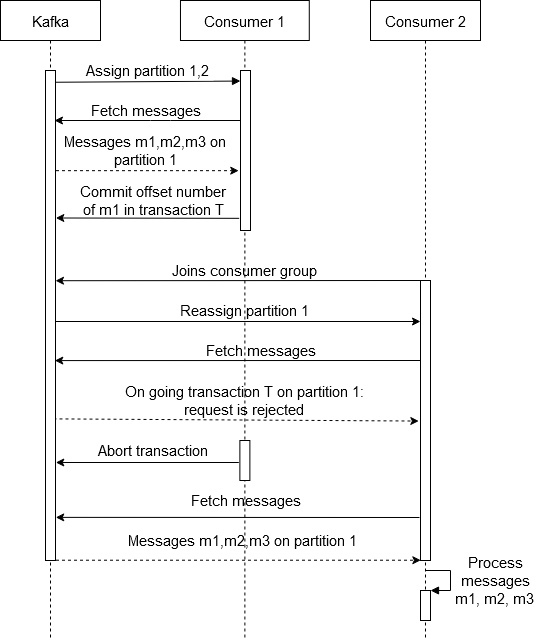
\includegraphics[width=11cm]{images/kafka-transaction-abort.png}
	\caption{Kafka transaction can prevent out-of-order processing of messages when transaction is aborted.}
	\label{fig:kafkatransactionabort}
\end{figure}
The problem of out-of-order processing is well prevented on Kafka. When a consumer in the consumer group commits the offset number of a message in a transaction, the entire partition to which the message belongs is locked and any other consumer in the same group cannot fetch new messages from this partition even when it is assigned as the new owner of the partition. Only when the ongoing transaction is either completed or aborted, new owner of the partition can start to pull new messages. On the old owner of the partition, after the ongoing transaction is finished, if there is any buffered message left from the last pull request, this application instance cannot continue to commit offset numbers for them because it now has the outdated metadata of the consumer group before the partitions reassignment. When this instance sends a new pulling requests to Kafka, it receives the latest metadata as well as only messages on the partition which it is currently assigned.

Therefore, at any time, only one consumer in a Kafka consumer group can process and commit offset numbers of messages on a partition. This mechanism of Kafka compromises the latency and availability to ensure the consistency when partition reassignment occurs. Moreover, all low-level implementation of transactions with Kafka producers and consumers as in this thesis is provided out-of-the-box with the Kafka Streams library. Users can utilize this library to focus only on the processing logic while still being able to achieve exactly-once semantics on Kafka with minimum configuration.

